\documentclass[11pt]{article}

\usepackage{fullpage}
\usepackage{amsfonts}
\usepackage{graphicx}
%\usepackage{color}
\usepackage[usenames, dvipsnames]{xcolor}
\usepackage{listings}
%\usepackage[titletoc,title]{appendix}
\usepackage{float}

\setcounter{secnumdepth}{5}

\makeatletter
\renewcommand\paragraph{\@startsection{paragraph}{4}{\z@}%
                                     {-3.25ex\@plus -1ex \@minus -.2ex}%
                                     {0.0001pt \@plus .2ex}%
                                     {\normalfont\normalsize\bfseries}}
\renewcommand\subparagraph{\@startsection{subparagraph}{5}{\z@}%
                                     {-3.25ex\@plus -1ex \@minus -.2ex}%
                                     {0.0001pt \@plus .2ex}%
                                     {\normalfont\normalsize\bfseries}}
\makeatother

\begin{document}
\newcommand{\HRule}{\rule{\linewidth}{0.5mm}}

\begin{titlepage}
\begin{center}

~\\[4cm]

\textsc{\Large \textsc{Utah State University} }\\[0.5cm]

% Title
\HRule \\[0.4cm]
{ \huge \bfseries Passive Tracking Device \\ -- Senior Project -- \\ Final Report \\[0.4cm] }

\HRule \\[1.5cm]

% Author
\noindent
\begin{minipage}{0.4\textwidth}
\begin{flushleft} \large
\textsc{ Dallin Marshall }
\end{flushleft}
\end{minipage}%
\begin{minipage}{0.4\textwidth}
\begin{flushright} \large
\textsc{ Computer Engineering }
\end{flushright}
\end{minipage}

\vfill

% Bottom of the page
{\large \today}

\end{center}
\end{titlepage}

% \textcolor{white, black, red, green, blue, cyan, magenta, yellow} {text}
% \section*{text}
% \subsection*{text}
% \subsubsection*{text}
% \begin{enumerate/itemize}
% \begin{center} \includegraphics[scale=0.4]{path.png}\end{center}
% \lstinputlisting[language=Matlab, basicstyle=\footnotesize, firstline=40, lastline=81]{Matlab_Diary.txt}
%
%\begin{figure}
%   \centering
%       \includegraphics[scale=0.4]{Circuit_Schmatic.png}
%   \caption{Circuit Schematic}
%   \label{fig:marker}
%\end{figure}
%
%   \begin{figure}[H]
%       \centering
%           \begin{minipage}[b]{0.45\linewidth}
%               \includegraphics[scale=0.3]{./Fan_Data/Data2/AllFansA.png}
%               \caption{All three Fans 100\%}
%               \label{fig:minipage1}
%           \end{minipage}
%           \quad
%           \begin{minipage}[b]{0.45\linewidth}
%               \includegraphics[scale=0.3]{./Fan_Data/Data2/Fans1_2.png}
%               \caption{Fans 1 and 2 100\%}
%               \label{fig:minipage2}
%           \end{minipage}
%   \end{figure}


\thispagestyle{empty}
\setcounter{tocdepth}{5}
\tableofcontents
%\pagebreak
\vspace{2cm}

\thispagestyle{empty}
\listoffigures
%\listoftables
\pagebreak

\pagenumbering{arabic}

\section{Executive Summary}
The PTD is a Passive Tracking Device that allows users to receive SMS messages updating them on the current location of an All Terrain Vehichle (ATV). Passive solutions differ
from active solutions in that they require less power and are less expensive for the users on a monthly service contract. This device is targeted for 
enterprise use to help track large fleects of ATVs. This document provides an overview of the components and methods used to create the PTD and discuss design tradeoffs during the design process. The PTD completed 
the specifications from the \textit{Specifcation Document} and was a valid proof of concept for future Passive Tracking Device development. 

The PTD is composed of four primary subsytems. These subsystems include the: Microcontroller, Cell Module, GPS Module, and Power Regulator. The microcontroller receives the raw
GPS data from the GPS Module, converts this data into a human friendly form, and composes and transmits an SMS message to a pre-determined cell number. For further details
see the Methods section of this document. 

Although originally developed for enterprise use throughout the design of the PTD it has been realized that the PTD can also function just as well for personal use for tracking
both ATVs and full-sized vehichles. The price of the PTD and cell service are inexpensive enough for the general public as well as small and large businesses. 
 
\section{Introduction}
There are many businesses that use ATVs (All Terrain Vehicles) to accomplish their work. These businesses range from contruction companies to civil
engineering firms, to the National Forest Service. Many times the larger the company the harder it is to manage the fleet of vehicles. The task of
keeping track of these vehicles is further compounded by human error as well as geographical isolation and dispersion of resources. These businesses
need a device that facilitates the management of their fleet. 

\subsection{Introduction}
There are many tracking solutions available for public and enterprise use but they generally all have the same problem. They are active tracking 
solutions. This means that the vehicle being tracked can only be tracked in real-time. The client of one of these active solutions could use the 
monitoring software to see on a map the location and movements of the vehicles in their fleet. While there are applications where 
active monitoring is necessary there are some major drawbacks to such a system. Three of the largest drawbacks are:
\begin{enumerate}
    \item Active systems require large amounts of power and physical space
    \item Active systems are quite costly
    \item There are applications that don't require real-time updates of vehicle location
\end{enumerate}
This means that the tracking bug itself is responsible for periodically transmitting it's location to the client. From the client's side, the client 
can only see the last known location of the vehicle. The PTD is a passive tracking solution that is targeted to counter these drawbacks of active 
solutions by functioning in low-power environments that do not require real-time updates and at a reasonable cost. By targeting markets that don't require 
active solutions the tracking bug can be made cheaper, smaller, more power efficient, and provide a cheaper solution overall for the customer.  
\footnote{See the Problem and Objectives sections of this document for information 
regarding this topic.}


\subsection{Problem}
The PTD is targeted at making this task considerably easier. 
The PTD, once installed in an ATV, uses the internal battery of the ATV to periodically transmit it's location to the managing individual. This will help 
monitor vehicle usage as well as recover vehicles in the event of theft.


\section{Methods}
In this section I will expound upon each of the sub-systems and explain in greater detail their function and components.
The Passive Tracking Device consists of four subsystems:
\begin{itemize}
    \item \textbf{Microcontroller} - I chose the Tiva-C TM4C123G for prototyping this project because it has plenty of serial
          UART communication modules as well as an internal 3.3 V generator that can be used to power the Copernicas 2 GPS Module. 
          It is also operates in a fairly low power range. 

    \item \textbf{Cell Module} - I chose the Adafruit FONA 1946 Cell Module. The FONA Cell Module was chosen because of it's ease of prototyping
          and compatability with all 2G and 3G GSM Cell Networks. It is also controlled via a UART communication module to send text messages. This Cell Module 
          also happened to be at the most attractive price point when compared to other Cell Modules. This Module makes use of the SIM 800L cell component
          which was previously looked at as a viable option for this project because of it's commonality in standard cellular devices. 
          \footnote{Included in this subsystem of the project it should be noted that a small lithium ion battery for transmission 
          power stability, an SMA ducbill cell antenna, and a uFL to SMA adapter are required to complete this subsystem.} 

    \item \textbf{GPS Module} - I chose the Trimble Copernicas 2 GPS Module. The Copernicas 2 GPS Module requires a 3.3 V voltage source for power and uses a serial UART 
          communication module operating at 4800 BOD to communicate it's location to other systems. \footnote{Note that this subsystem requires a GPS antenna that
          uses the common SMA connector. This is in addition to the Cell Module antenna because the two antennas operate on very different bands of communication.} 

    \item \textbf{Power Regulator} - I chose to purchase the DROK Adjustable Switching Voltage Regulator for the purpose of prototyping this project. This DROK Regulator makes
          use of the Texas Instruments LM2596 Switching Regulator which I had previously chosen as my target regulator. This prefabricated module made the task of
          prototyping manageable. I also chose this power regulator because of it's adjustable functions that would later allow me to use it on other projects and 
          because it can source a maximum of 3 amps. \footnote{The PTD does not come close to 3 AMPs but I wanted this feature for future prototyping} 
\end{itemize} 

\subsection{Microcontroller} 
The Tiva-C microcontroller operates at 16 MHz by default. I chose to use this default setting of 16 MHz because a higher clock frequency was not necessary and 
if I had increased it then it would have required more power. I chose to activate three of the available eight UART communication modules for the PTD. I needed 
one UART module for each of the following: receive GPS location from GPS Module, send formatted GPS location as a message to the Cell Module for SMS tranmission,
and one to allow the client easy cell number destination configuration for text messages. I chose to use interrupts instead of pulling a status bit for each of
the UART modules to make code more understandable and maintainable. To better understand how the microcontroller is connected to the other components of the PTD please see
Figure: \ref{fig:wiring_diagram}. 

\begin{figure}
    \centering
        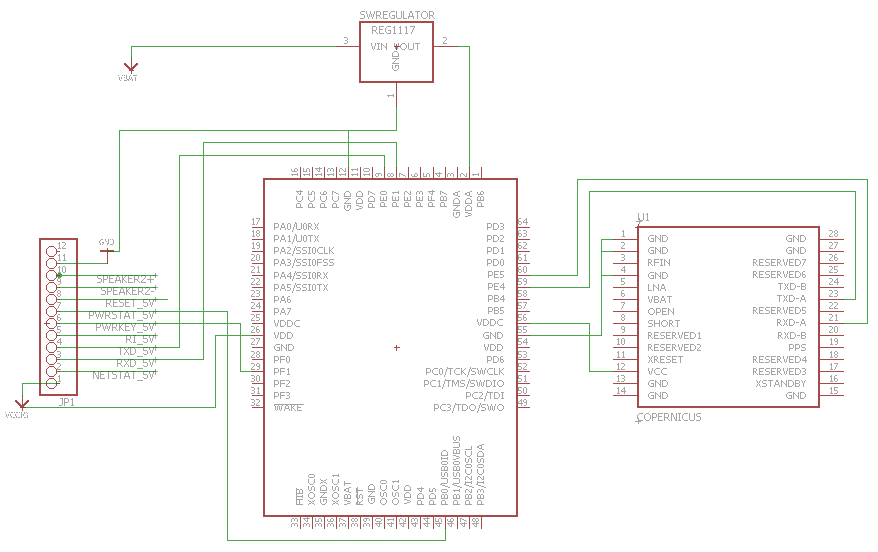
\includegraphics[scale=0.5]{../documentation/PTD_Eagle_Schematic.png}
    \caption{PTD Wiring Diagram}
    \label{fig:wiring_diagram}
\end{figure}


\subsection{Cell Module}
The Adafruit FONA 1946 Cell Module has a BOD detecting UART module that detects the transmission speed from the communicating system and 
replies at the same speed. Because of this convenient feature I used 4800 BOD to communicate with the Cell Module because the GPS Module requires 4800 BOD. This 
allowed me to simplify my configuration for all UART modules by using the same speed configuration. This module uses the common AT command set to
control cellular functions. To connect to a valid US cell network a pre-paid T-Mobile SIM card was purchased because of the low price point and lack of annual contract. 
This SIM card costs 10 cents per message. With this cost the PTD can send an SMS message update once every 8 hours for only 30 cents a day. This is much cheaper than other options on 
the market today. 


\subsection{GPS Module}
The Trimble Copernicas 2 GPS Module works well because of it's easy "plug and play" set up. Upon receiving power this module initializes and after a few seconds begins
to transmit locational data every second at a rate of 4800 BOD. The microcontroller is responsible for parsing this string and translating it into a more human readable GPS location 
to be sent via SMS to the client.  


\subsection{Power Regulator}
I selected the LM2596 Texas Instruments Switching Regulator because of it's low-idle power loss as well as it's voltage range and current operating output. When looking
to buy the individual LM2596 components the spec sheet made it clear that external capacitors, inductors, diodes, resistors, and potentiometers needed to be purchased separately
in their desired configuration in order to correctly control the output voltage of the Switching Regulator. To avoid this headache during the prototyping phase I opted
to buy the DROK Switching Regulator which comes preassembled with the desired components. Both the microcontroller and the Cell Module require a 5V source to operate.
The LM2596 regulator provides this necessary voltage regulation from a typical ATV battery which normally are 12V 11Ah batteries. From the beginning switching regulators were
preferred over linear regulators due to the improved power characteristics from a switching power regulator. The constant power dissipation of a linear regulator makes them 
undesirable for low power operation.\footnote{This is a part of the PTD that would need to be custom manufactured on a large scale manufacturable PCB}   


\section{Results}
This section outlines the requirements and results of the tests for those requirements.

\subsection{Item Definitions}
The PTD consists of 4 main subsystems, namely:
\begin{itemize}
    \item Cell Network Interface
    \item Global Positioning System
    \item Controller Circuit
    \item Power Converter/Regulator
\end{itemize}
The PTD system will be a passive system, meaning that the PTD will power down to a very low power state while not in use. At an appointed 
trigger it will power up and transmit it's location to the PTDs owner via a cell network. There is no plan for the owner of the PTD to be able to 
activate the device externally. The PTD shall opperate in this power-up, transmit location, power-down sequence.

The PTD designed follows the block diagram in Figure: \ref{fig:block_diagram} which shows that all sub-system functions have been used to complete with the clients expectations.

\subsubsection{Interface Description/Functional Block Diagram}
The PTD used a micro-controller to act as a intermediary logic location for the signals between the GPS and Cell Module. All UART communication used in the project is configured to run
at 4800 BOD. The block diagram of the PTD can be seen in Figure: \ref{fig:block_diagram}.
\begin{figure}
    \centering
        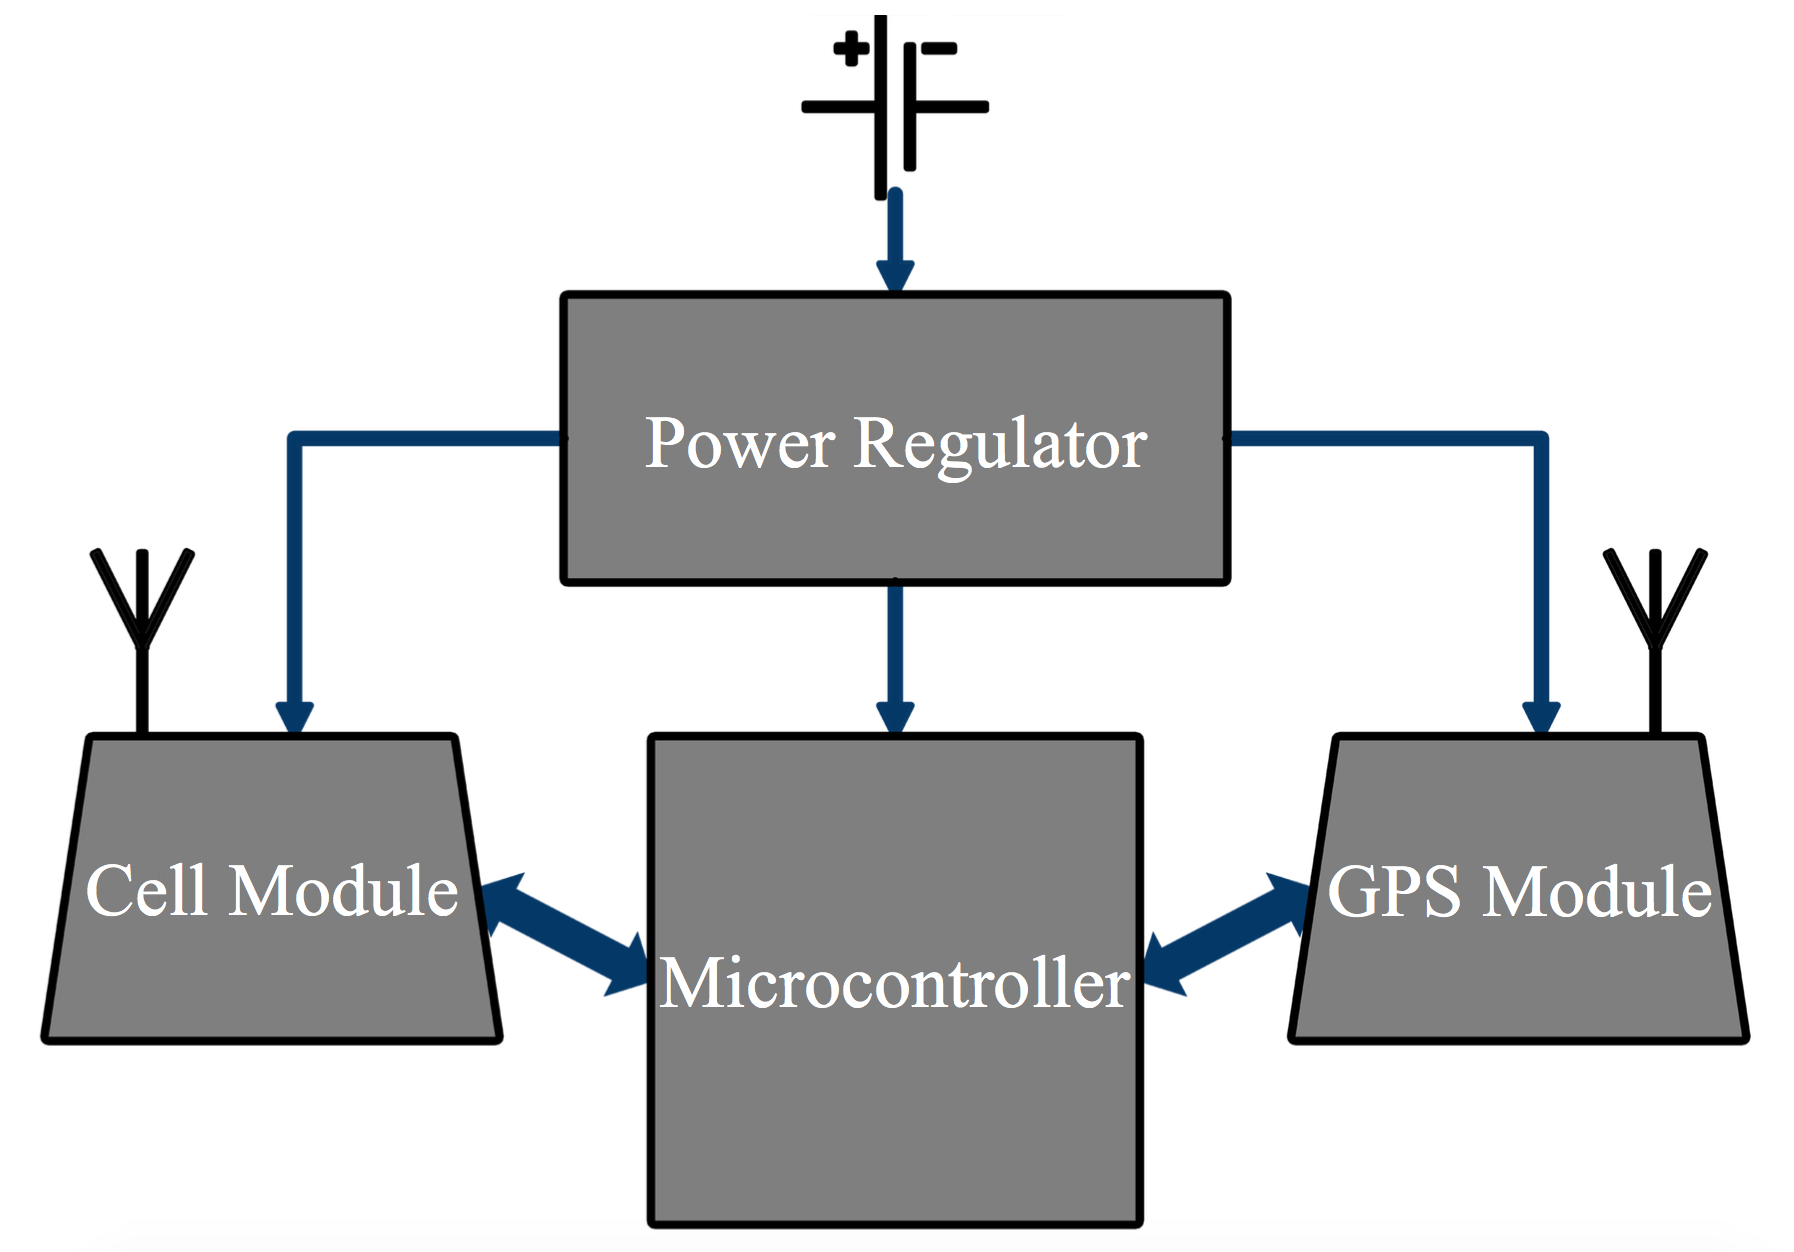
\includegraphics[scale=0.25]{../documentation/block_diagram.png}
    \caption{PTD Block Diagram}
    \label{fig:block_diagram}
\end{figure}

\subsection{Characteristics}
The following section provides a technical summary of the PTD's characteristics.

\subsubsection{Performance Characteristics}
To comply with the specification document the PTD must complete tests or justify adaquitly that the device will complete the tests at a later stage of developement.

\paragraph{Physical Characteristics}
The PTD shall meet the following physical requeirements:
    \subparagraph{Form Factor}  The PTD shall conform to the following form factor: 16cm by 8cm by 5cm.
        \begin{description}
            \setlength{\itemindent}{1em}
            \item{\textbf{Test} -} The PTD shall be placed in an small box of dimention stated in requirements.
            \item{\textbf{Result} -} \textcolor{Red}{Failed:} The PTD measures 10.5cm by 6.5cm by 5.5cm. These dimensions do not fit inside a box of the specified dimensions. 
        \end{description}

\paragraph{Electrical Characteristics}
The PTD shall meet the following electrical requirements:
    \subparagraph{Power Constraints}  The PTD shall operate using the power provided by a standard ATV battery, specifically, 12V 11Ah battery.
        \begin{description}
            \setlength{\itemindent}{1em}
            \item{\textbf{Test} -} The PTD shall function with only the power provied by an ATV battery. The PTD shall also be tested while the ATV's engine is actively running and under normal operation.
                \hspace*{4cm}requirements.
            \item{\textbf{Result} -} \textcolor{Green}{Passed:} After hooking the PTD to the ATv it functioned properly using only the ATV battery.
        \end{description}
    \subparagraph{Prototype Connections}  For the purposes of proof of concept the PTD may make use of a breadboard to connect the components.
        \begin{description}
            \setlength{\itemindent}{1em}
            \item{\textbf{Test} -} The PTD shall have connections that function, The design of these connections is not specified in the \textit{Specification Document}.
                \hspace*{4cm}requirements.
            \item{\textbf{Result} -} \textcolor{Green}{Passed:} The manner of connecting the components together was not specified and therefore is an automatic pass. 
        \end{description}

\subsubsection{Environmental Characteristics}

\paragraph{Natural Characteristics}
The PTD shall meet the following natural evironmental characteristics. The PTD shall meet the requirements of this specification during and 
after exposure to any combination of any of the following natural environments. The PTD may be packaged to precluded exposure to any 
environments that would control the design.
    \subparagraph{Temperature Rating}  The PTD shall function between 0$^{\circ}$ C and 40$^{\circ}$ C.
        \begin{description}
            \setlength{\itemindent}{1em}
            \item{\textbf{Test} -} The PTD shall be tested for full functionality at both ends of the temperature spectrum.
                \hspace*{4cm}requirements.
            \item{\textbf{Result} -} \textcolor{Green}{Passed:} The PTD was tested at the high of 40$^{\circ}$ C and the low of 0$^{\circ}$ C. It passed under both conditions. 
        \end{description}

\paragraph{Induced Environment Characteristics}
The PTD shall meet the following induced evironmental characteristics. The PTD shall meet the requirements of this specification during 
and after exposure to any combination of any of the following induced environments. The PTD may be packaged to precluded exposure to any 
environments that would control the design.
    \subparagraph{Shock Test}  The PTD shall withstand mechanical shocks of 3 ft drop test 5 times onto concrete.
        \begin{description}
            \setlength{\itemindent}{1em}
            \item{\textbf{Test} -} The PTD shall function after the drop tests.
                \hspace*{4cm}requirements.
            \item{\textbf{Result} -} \textcolor{Green}{Passed:} The PTD functions after drop test. 
        \end{description}
    \subparagraph{Vibration Test}  The PTD shall withstand vibrations of 1 ocilations per second with an amplitude of 1.5cm for 1 hour.
        \begin{description}
            \setlength{\itemindent}{1em}
            \item{\textbf{Test} -} The PTD shall function after the vibration test is performed.
                \hspace*{4cm}requirements.
            \item{\textbf{Result} -} \textcolor{Green}{Passed:} The PTD functions after vibration test. 
        \end{description}
    \subparagraph{Dust Test}  The PTD shall function in a dusty environment, specifically, the shock and vibration tests shall be repeated 
after 15 grams of fine sand is applied to the device. 
        \begin{description}
            \setlength{\itemindent}{1em}
            \item{\textbf{Test} -} The PTD shall function after the dust test is performed.
                \hspace*{4cm}requirements.
            \item{\textbf{Result} -} \textcolor{Green}{Passed:} Shock and Vibration tests were repeated after applying dust and PTD continues to function. 
        \end{description}

\subsection{Electromagnetic Interference}
The EMI shall be measured and shall meet the requirements found in 
\begin{itemize}
    \item The United States (US) FCC Part 15-2008.
    \item Canada's Industry Canada ICES-003:2004 Issue 4.
\end{itemize}
This is to allow for legal manufacturing and usage is the United States and Canada.

\section{Discussion}
This section is designed to discuss the \textit{Results} section of this document. The methods of testing and possible design modifications resulting from 
testing will also be covered here.

\subsection{Characteristics}
The following section provides a technical summary of the PTD's characteristics pertaining to the \textit{Results} section.

\subsubsection{Performance Characteristics}
To comply with the specification document the PTD must complete tests or justify adaquitly that the device will complete the tests at a later stage of developement.

\paragraph{Physical Characteristics}
The PTD shall meet the following physical requeirements:
    \subparagraph{Form Factor}  The PTD shall conform to the following form factor: 16cm by 8cm by 5cm. \newline ~ \newline
        This is the single section from the \textit{Specification Document} that was not achieved durring the testing phase of this project. After talking to the client
        it was desided that the reason for the specified dimmensions was to allow for a prototyped solution. When this project moves to the next phase of developement where
        custom PCBs will be manufactured with all of the components on the same board the form factor will be well within the needed size constraints for this project.
        It was therefore decided not judge this project as a failure as a result of failing to meet the form factor requirements.

\paragraph{Electrical Characteristics}
The PTD shall meet the following electrical requirements:
    \subparagraph{Power Constraints}  The PTD shall operate using the power provided by a standard ATV battery, specifically, 12V 11Ah battery. \newline ~ \newline
        The PTD was designed with these power constraints in mind and it is able to operate given an ATV battery. It should be noted that the PTD 
        expects that the ATV battery is in good working condition. Oridinally when testing the PTD the Battery functioned perfectly. This was back in September. As temperatures 
        in Logan began to drop the upon ingition of my motorcycle the PTD began to reset itself. This was caused by the momentary drop in the power provided to the PTD from the 
        battery. This is not a flaw in the PTD but an example of the importance of using a ATV battery in good working condision. My Motorcycle batter is about 5 years old and 
        should soon be replaced. 
    \subparagraph{Prototype Connections}  For the purposes of proof of concept the PTD may make use of a breadboard to connect the components. \newline ~ \newline
        Originally the PTD was prototyped using a bread board but for reasons that will be discussed in the \textit{Drop Test} section the design of the prototype was 
        altered to use perf-board to better secure connections between components. This completes and exceeds the specifications.

\subsubsection{Environmental Characteristics}
The following sections outlines the Environmental Characteristics associated with the PTD. 

\paragraph{Natural Characteristics}
The PTD shall meet the following natural evironmental characteristics. The PTD shall meet the requirements of this specification during and 
after exposure to any combination of any of the following natural environments. The PTD may be packaged to precluded exposure to any 
environments that would control the design.
    \subparagraph{Temperature Rating}  The PTD shall function between 0$^{\circ}$ C and 40$^{\circ}$ C. \newline ~ \newline
        These tests were done at very different times of the developement. The hot test of 40$^{\circ}$ C was done in late September and the cold test of 0$^{\circ}$ C was 
        done in December. To complete with the hot test I created a chamber out of a cardboard box. I used my wifes hair dryer as the heat source, and here instant read cooking 
        thermometer to verify the temperature. I then ran the GPS antena out the window and verified that at 40$^{\circ}$ C, which is 104$^{\circ}$ F, the tracking bug functioned. The cold test
        was a little less involved. I waited until a cold winter night and took the PTD out to my patio and left it for 3 hours. The PTD functioned fine durring and after each of these tests.

\paragraph{Induced Environment Characteristics}
The PTD shall meet the following induced evironmental characteristics. The PTD shall meet the requirements of this specification during 
and after exposure to any combination of any of the following induced environments. The PTD may be packaged to precluded exposure to any 
environments that would control the design.
    \subparagraph{Shock Test}  The PTD shall withstand mechanical shocks of 3 ft drop test 5 times onto concrete. \newline ~ \newline
        This test was pretty straight forward. My plan was to drop the PTD on my kitchen floor which is concrete as see what happend. I was a little hesitant because at the point of this 
        testing the PTD was still developed using a bread board. Upon dropping the PTD the components and wires practically exploded out of the bread board. They still functioned after 
        the reconnection of all the components but because of this experiment and to make the PTD more compact and clean looking I used perf-board to create a new more permainant structure for the 
        PTD. The rest of the drop tests were completed after the change of structure and were more successful.
    \subparagraph{Vibration Test}  The PTD shall withstand vibrations of 1 ocilations per second with an amplitude of 1.5cm for 1 hour. \newline ~ \newline
        This test was the worst test for me to complete because it took my active attention for a solid hour. Luckily I used this time to catch up on one of my favorite tv shows during the time that 
        I was shaking the PTD. The PTD functioned fine after this test. This test was done after the perf-board modifications. \footnote{It is actually a lot harder than expected to shake something 
        for an hours straight.}
    \subparagraph{Dust Test}  The PTD shall function in a dusty environment, specifically, the shock and vibration tests shall be repeated 
        after 15 grams of fine sand is applied to the device. \newline ~ \newline 
        Like most American households I didn't have a food scale available so I used a little math to estimate the volume of dirt necessary to represent 15 grams. I know that 4 grams of sugar is about
        one teaspoon. Using this rough estimate I used my wife's measuring spoons\footnote{I don't think my wife enjoys it when my experiments infringe on her cooking utensils.} to gather 4 
        teaspoons of dirt which I placed in a box with the PTD. I then closed up the box and repeated the shock and vibrations tests. I modified the vibrations test this time to avoid having to manually shake 
        the PTD for an hour, so I placed the PTD and dust box on our dryer and did some laundry. This simulated the same vibration time as the manual test did earlier in the testing phase. I then used an air 
        compressor to clean off the PTD before verifying that the PTD worked and function was not degraded by the stress.

\subsection{Electromagnetic Interference}
The PTD was create with components that all comply with the electromagnetic interference standards described in 
\begin{itemize}
    \item The United States (US) FCC Part 15-2008.
    \item Canada's Industry Canada ICES-003:2004 Issue 4.
\end{itemize}
and because the normal function of the components was not changed the completed project also conforms to with these standards without needing to be tested.

\subsection{Project Schedule and Budget}


\section{Conclusion}
The PTD functions well as a passive tracking solution. It also completed all of the specifications from the spec document. The PTD will also be much less space intensive when all components are manufactured on a single
custom PCB. A year ago when I began looking at possible component candidates for this project there were not microcontrollers with cell functionality on a single board, but this is not the case today. 
There are now solutions such as the Particle Electron that are a microcontroller couples with a cell module on the same board. This would allow easier integration into a tracking device as well as lower
the power necessary for the device. It would also reduce the cost. Before moving to large scale  manufacturing of the PTD these new alternative components should be explored for possible cost and functionality
benefits.

To complete this project I decided to make use of the Code Composer Studio (CCS) development suite. I chose CCS primarily because I had never worked with it before and decided to make use of the opportunity 
to become familiar with another Integrated Design Environment (IDE). This proved to be helpful and detremental to this project's success. It turns out that CCS does not play well with multi-file projects and
that it incorrectly performs dynamic memory operations on the microcontroller even when it advertises that it does these operations correctly. This caused me much time and frustration debugging operations that
were syntactically correct but that CCS was implementing incorrectly. To fix these problems I re-wrote many parts of this project in later phases. I think that the PTD is a valid proof of concept of cheap, low 
power, passive tracking devices that could be used to monitor personal and enterprise vehichles in a cost effective manner. Overall I rate this project as a success.   

\end{document}


